\subsection{Sviluppo}

\subsubsection{Descrizione e Scopo}
Il processo di sviluppo rappresenta l’insieme delle attività necessarie per realizzare il prodotto software, garantendo il rispetto dei requisiti e delle scadenze concordate con il proponente. Questo processo si articola in diverse fasi fondamentali, quali l'analisi dei requisiti, la progettazione, la codifica, l'integrazione, e la verifica, assicurando che ogni fase contribuisca al raggiungimento degli obiettivi prefissati.
Le linee guida descritte in questa sezione sono volte a strutturare il lavoro in modo chiaro e uniforme, promuovendo la qualità del prodotto finale. Seguendo standard solidi e definiti, nel caso specifico l'ISO/IEC 12207:1995, si crea un ambiente di lavoro orientato a garantire la coerenza nei metodi utilizzati e il rispetto delle aspettative.
L'obiettivo è consegnare un prodotto software di alta qualità, che soddisfi le esigenze richieste, rispettando le tempistiche e garantendo il successo del progetto.\\

\subsubsection{Analisi dei Requisiti}
    \paragraph{Descrizione e Scopo}
    L’analisi dei requisiti è la prima fase cruciale del processo di sviluppo software. Lo scopo principale di questa fase è definire con chiarezza le funzionalità e le caratteristiche che il sistema dovrà offrire, in base alle necessità degli utenti. Per raggiungere tale obiettivo, è essenziale stabilire una comunicazione efficace con il proponente, assicurandosi che tutte le esigenze siano documentate e validate. Questo processo permette di chiarire gli obiettivi del prodotto, identificare i vincoli operativi e fornire ai Progettisti le informazioni necessarie per sviluppare un’architettura coerente e un design adeguato. Il risultato di questa attività è formalizzato nel documento \textit{Analisi\_dei\_Requisiti.pdf}, redatto dagli Analisti, che contiene una descrizione dettagliata degli obiettivi del prodotto, delle funzionalità previste, delle caratteristiche degli utenti e delle tecnologie coinvolte. Include inoltre una sezione dedicata ai casi d’uso, che descrivono le interazioni tra gli attori esterni e il sistema. \newline 
    Infine, l’analisi dei requisiti contribuisce a migliorare la comunicazione tra tutti gli stakeholder, agevola la pianificazione del progetto in termini di tempistiche e costi e fornisce un riferimento chiaro per le attività di verifica e test.\\

    \paragraph{Casi d'uso}
    I casi d’uso rappresentano scenari concreti che descrivono come gli utenti e altri attori interagiranno con il sistema per raggiungere obiettivi specifici. Questi scenari aiutano a identificare requisiti chiave e prevenire malintesi. È importante sottolineare che i diagrammi dei casi d’uso non si concentrano sui dettagli implementativi. Il loro scopo è quello di rappresentare la funzionalità del sistema esclusivamente dal punto di vista esterno, evidenziando come esso interagisce con gli attori e soddisfa le loro esigenze.\\
    \medskip
    Ogni caso d'uso ha le seguenti caratteristiche:
    
    \begin{itemize}
    \item \textbf{Identificativo}:
    \begin{quote}
    \textbf{UC [Numero caso d’uso] . [Numero sottocaso d’uso] - [Titolo]}
    \end{quote}
    Dove:
    \begin{itemize}
        \item \textbf{Numero caso d’uso}: ID relativo al caso d'uso principale;
        \item \textbf{Numero sottocaso d’uso}: ID relativo allo specifico sottocaso d'uso (se applicabile);
        \item \textbf{Titolo}: descrizione breve ed esplicativa;
    \end{itemize}

    \item \textbf{Attore principale}: Entità esterna che interagisce attivamente con il sistema per raggiungere uno scopo, ad esempio un utente specifico o un altro sistema esterno;
    \item \textbf{Attore secondario}: Eventuale entità esterna invocata dal sistema per fornire un supporto, in modo da soddisfare il bisogno dell’attore principale;
    \item \textbf{Descrizione}: Breve descrizione della funzionalità del caso d’uso;
    \item \textbf{Scenario principale}: Sequenza di eventi che si susseguono da quando un attore inizia ad interagire con il sistema;
    \item \textbf{Precondizioni}: Descrizione dello stato del sistema necessario per attivare il caso d’uso;
    \item \textbf{Postcondizioni}: Descrizione dello stato del sistema al completamento del caso d’uso;
    \item \textbf{Estensioni}: Eventuali scenari alternativi, descritti in questa sezione se presenti;
    \item \textbf{User story associata}: Funzionalità descritta dal punto di vista dell'utente, scritta in linguaggio naturale perché risulti semplice e comprensibile. Definita nella forma seguente: \newline
    Come [utente], desidero poter [funzionalità] per [valore aggiunto].
\end{itemize}

\paragraph{Diagrammi dei casi d'uso} 
I diagrammi dei casi d'uso sono strumenti visivi che rappresentano le funzionalità del sistema dal punto di vista dell'utente. Mostrano come gli attori esterni (utenti, dispositivi, altri sistemi) interagiscono con il sistema, senza entrare nei dettagli tecnici. Il loro obiettivo principale è descrivere le interazioni tra attori e sistema, facilitando la comprensione dei requisiti funzionali e la comunicazione tra gli stakeholder. Ogni caso d'uso descrive una sequenza di azioni che un attore compie per raggiungere un obiettivo specifico. Questi casi sono interconnessi e rappresentano i flussi di lavoro principali, evidenziando come l'utente interagisce con il sistema. I diagrammi non trattano i dettagli implementativi, ma si concentrano sulle funzionalità, trattando il sistema come un "black box" esterno.\\
\medskip Di seguito sono elencati i principali componenti di un diagramma dei casi d’uso:

\begin{itemize}
    \item \textbf{Attori}\\
        Gli attori sono entità esterne al sistema che interagiscono con esso per utilizzare le sue funzionalità. Possono essere utenti umani, altri sistemi software, dispositivi, macchine o organizzazioni. Un caso d'uso definisce una specifica funzionalità che il sistema fornisce agli attori, senza entrare nei dettagli implementativi. Nel diagramma dei casi d'uso, gli attori sono rappresentati da figure stilizzate posizionate all'esterno del rettangolo che delinea il sistema, e ciascuno è identificato da un’etichetta con il suo nome.
        \begin{figure}[H]
        \centering
        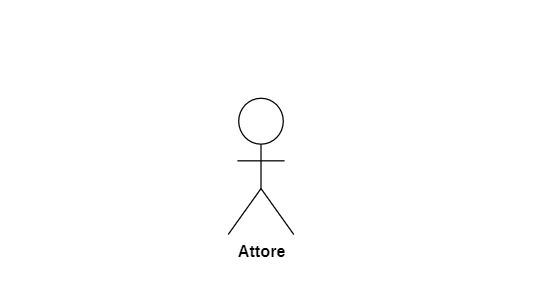
\includegraphics[width=0.45\textwidth]{Attore.PNG}
        \caption{Rappresentazione di un attore.}
        \end{figure}

        \item \textbf{Casi d'uso}\\
        Ogni caso d’uso identifica una specifica azione o funzionalità offerta dal sistema, con cui l’attore può interagire. I casi d'uso sono collegati tramite una linea continua agli attori che hanno accesso a quella funzionalità, creando una chiara relazione tra gli utenti e le azioni che possono compiere. Nel diagramma dei casi d’uso, ogni caso è rappresentato da una forma ovale contenente un ID univoco e un titolo esplicativo.
        \begin{figure}[H]
        \centering
        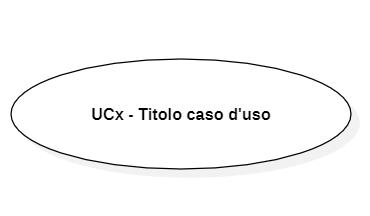
\includegraphics[width=0.35\textwidth]{UC.PNG}
        \caption{Rappresentazione di un caso d'uso.}
        \end{figure}

        \item \textbf{Sottocasi d'uso}\\
        Un sottocaso d’uso rappresenta una versione più dettagliata di un caso d’uso  generico. Esso offre un livello di dettaglio più approfondito sulle funzionalità o sui particolari scenari di utilizzo rispetto al caso d’uso principale. Non è obbligatorio per un caso d'uso possedere uno o più sottocasi.
        \begin{figure}[H]
        \centering
        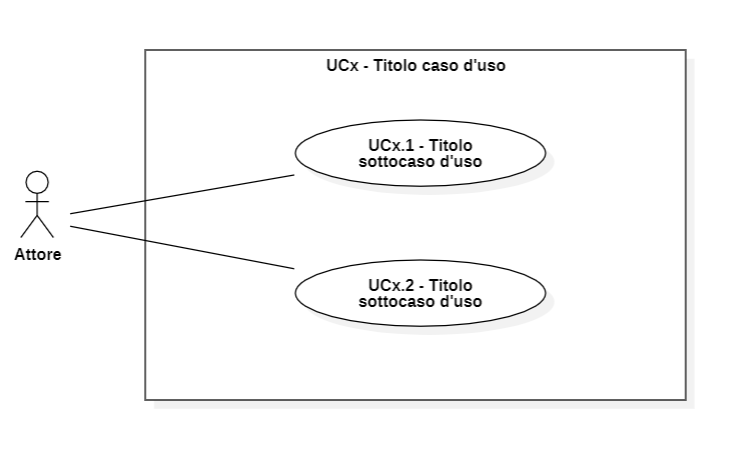
\includegraphics[width=0.6\textwidth]{SottocasoD'Uso.PNG}
        \caption{Rappresentazione di un sottocaso d'uso.}
        \end{figure}

        \item \textbf{Sistema}\\
         Il sistema viene rappresentato con un rettangolo all'interno del quale vengono collocati i casi d'uso. All'esterno del rettangolo sono invece posizionati i vari attori.
        \begin{figure}[H]
        \centering
        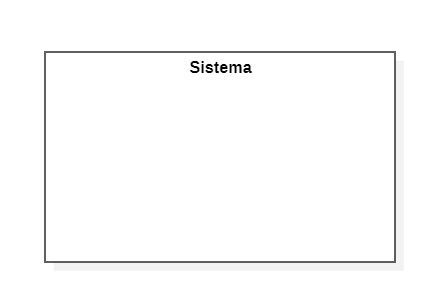
\includegraphics[width=0.5\textwidth]{Sistema.PNG}
        \caption{Rappresentazione di un sistema.}
        \end{figure}

        \item \textbf{Associazione}\\
        Una linea di associazione stabilisce una connessione tra un attore e un caso d'uso quando l'attore è coinvolto nell'attività descritta dal caso d'uso. Questo collegamento visivo rappresenta il ruolo dell'attore nell'attivare o nell'utilizzare una specifica funzionalità del sistema.
        \begin{figure}[H]
        \centering
        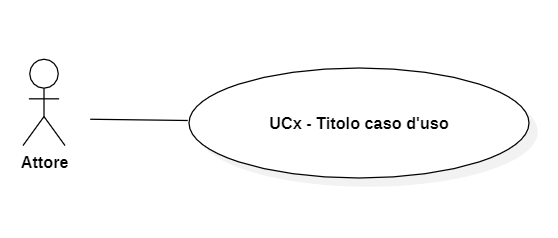
\includegraphics[width=0.5\textwidth]{Associazione.PNG}
        \caption{Rappresentazione di un sistema.}
        \end{figure}

        \item \textbf{Generalizzazione (attori)}\\
        La generalizzazione tra attori rappresenta una relazione gerarchica in cui un attore specializzato (figlio) eredita comportamenti e caratteristiche da un attore base (genitore). Questo meccanismo aiuta a organizzare gerarchicamente gli attori nei diagrammi dei casi d’uso, definendo i casi d'uso che un attore può utilizzare e che sono anche disponibili per gli attori più specializzati. La generalizzazione viene rappresentata con una linea solida e una freccia vuota che va dall'attore figlio all'attore genitore, indicando la direzione dell'eredità.
        \begin{figure}[H]
        \centering
        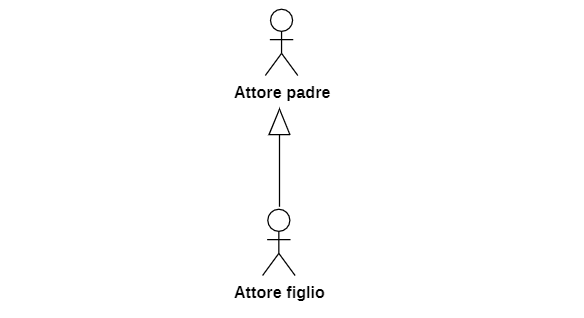
\includegraphics[width=0.6\textwidth]{GeneralizzazioneAttori.PNG}
        \caption{Rappresentazione di un sistema.}
        \end{figure}

        \item \textbf{Inclusione}\\
        La relazione di inclusione indica quando un caso d'uso (includente) comprende l'esecuzione di un altro caso d'uso (incluso). Quando un attore interagisce con il caso d'uso includente, il caso d'uso incluso viene eseguito automaticamente come parte di quest'ultimo. Questa relazione è utile per il riutilizzo delle funzionalità e per evitare la duplicazione delle stesse logiche in più casi d'uso. La relazione di inclusione viene rappresentata da una freccia tratteggiata che collega il caso d'uso incluso al caso d'uso includente.
        \begin{figure}[H]
        \centering
        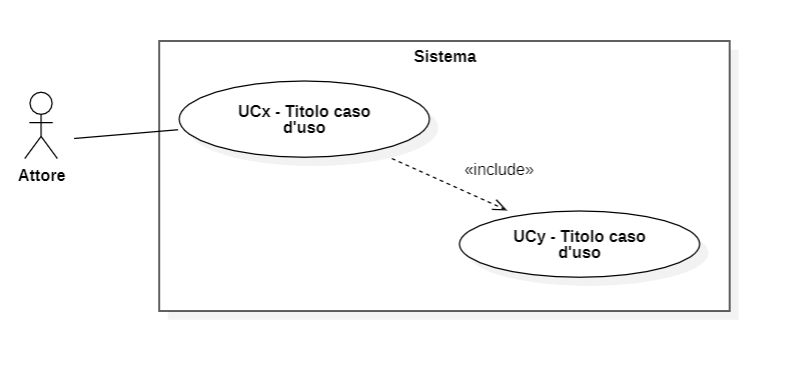
\includegraphics[width=0.6\textwidth]{Inclusione.PNG}
        \caption{Rappresentazione di un sistema.}
        \end{figure}

        \item \textbf{Estensione}\\
        La relazione di estensione indica quando un caso d'uso (estendente) può modificare o arricchire il comportamento di un altro caso d'uso (esteso) in determinate circostanze. Questa relazione viene utilizzata quando un evento o una condizione porta il flusso del caso d'uso a deviare dallo scenario principale verso uno scenario alternativo, come nei casi di errore, ma mantenendo le stesse precondizioni del caso d'uso principale. La relazione di estensione è rappresentata da una freccia tratteggiata che collega il caso d'uso estendente al caso d'uso esteso.
        \begin{figure}[H]
        \centering
        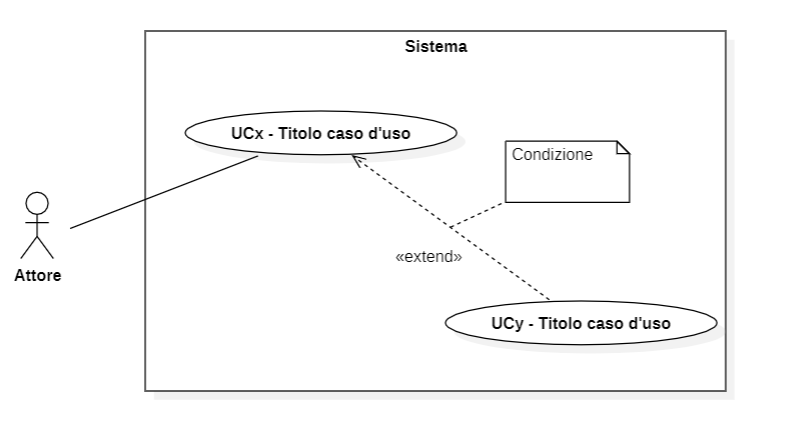
\includegraphics[width=0.6\textwidth]{Estensione.PNG}
        \caption{Rappresentazione di un sistema.}
        \end{figure}

        \item \textbf{Generalizzazione (casi d'uso)}\\
        La generalizzazione nei diagrammi dei casi d’uso rappresenta una relazione di ereditarietà tra casi d’uso, in cui un caso d’uso più specifico eredita il comportamento da un caso d’uso più generico. Questa relazione è utile per definire funzionalità più dettagliate, ed è simboleggiata da una linea con una freccia vuota che va dal caso d'uso specifico al caso d'uso generico.
        \begin{figure}[H]
        \centering
        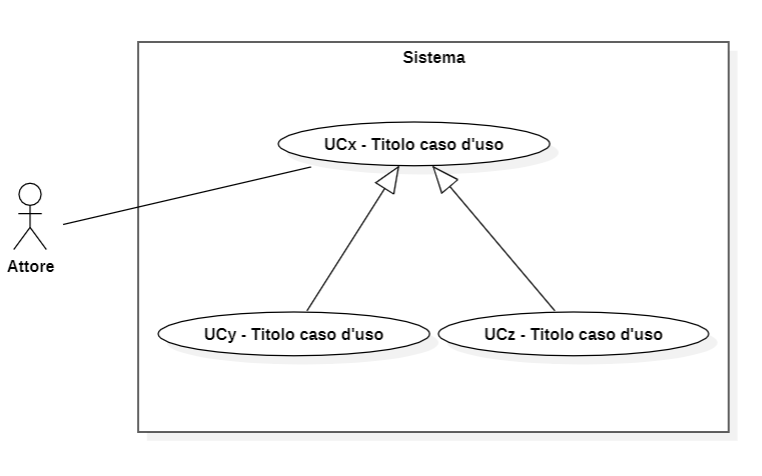
\includegraphics[width=0.6\textwidth]{GeneralizzazioneUC.PNG}
        \caption{Rappresentazione di un sistema.}
        \end{figure}
\end{itemize}

    \paragraph{Requisiti}
    I requisiti di un prodotto software sono specifiche documentate che delineano le funzionalità che il sistema deve soddisfare. Essi fungono da guida per lo sviluppo, il testing e la validazione del prodotto, garantendo che risponda alle esigenze degli utenti e agli obiettivi del progetto. Ogni requisito deve essere definito con precisione, e riflettere pienamente le attese del cliente o del proponente.\newline
    I requisiti si suddividono in tre diverse tipologie:
    \begin{itemize}
        \item \textbf{Requisiti funzionali (F)}: Specificano le funzionalità che il sistema deve essere in grado di svolgere, descrivendo le azioni principali e le informazioni che fornisce;
        \item \textbf{Requisiti di qualità (Q)}: Definiscono standard relativi alle prestazioni, affidabilità, sicurezza e altri criteri di qualità che il sistema deve rispettare;
        \item \textbf{Requisiti di vincolo (V)}: Rappresentano restrizioni o condizioni imposte al progetto, come vincoli tecnologici o normativi.
        \item \textbf{Requisiti prestazionali (P)}: Descrivono le capacità o le prestazioni minime richieste, come tempi di risposta, scalabilità o capacità di carico;
    \end{itemize}

    Ogni requisito è composto da:
    \begin{itemize}
    \item \textbf{Identificativo}: Un codice univoco nel formato:
    \begin{quote}
    \textbf{R[{Importanza}][{Tipologia}] X}
    \end{quote}
    Dove:
    \begin{itemize}
        \item \textbf{Importanza}:
        \begin{itemize}
            \item \textbf{O}: Obbligatorio. Essenziale per soddisfare le esigenze del proponente;
            \item \textbf{D}: Desiderabile. Utile ma non prioritario, può essere implementato in seguito;
            \item \textbf{P}: Opzionale. Aggiunge valore al prodotto, ma può essere tralasciato per motivi di costo o tempistica;
        \end{itemize}
        \item \textbf{Tipologia}:
        \begin{itemize}
            \item \textbf{F}: Funzionale;
            \item \textbf{Q}: Qualità;
            \item \textbf{V}: Vincolo;
            \item \textbf{P}: Prestazionale;
        \end{itemize}
        \item \textbf{X}: Numero progressivo per ogni requisito aggiunto;
    \end{itemize}
    \item \textbf{Descrizione}: Una descrizione dettagliata che spiega la caratteristica richiesta al sistema;
    \item \textbf{Fonte}: L'origine del requisito;
    \item \textbf{Casi d’uso associati}: Un elenco di casi d'uso che forniscono il contesto operativo per il requisito;
    \end{itemize}

    Alcuni requisiti, pur non avendo un identificativo, vengono documentati per assicurare la loro tracciabilità. Questi comprendono:
    \begin{itemize}
        \item \textbf{Requisiti d’ambiente}: 
        Specificano le condizioni e le risorse necessarie per sviluppare, testare e implementare il software;
        \item \textbf{Requisiti di sicurezza}: 
        Delineano le misure e i comportamenti richiesti per proteggere il sistema da minacce;
        \item \textbf{Requisiti di performance}: 
        Definiscono i livelli di prestazione richiesti, come velocità di elaborazione o capacità di gestione del carico;
    \end{itemize}

    \paragraph{Metriche}
    %da completare e inserire tabella%

\subsubsection{Progettazione}

    \paragraph{Descrizione e Scopo}     
    La progettazione, o design, è un'altra fase cruciale del processo di sviluppo software che ha l'obiettivo di tradurre i requisiti individuati durante la fase di analisi in una struttura architetturale definita. Questa attività definisce in dettaglio i vincoli e le caratteristiche del prodotto semplificando la pianificazione e la suddivisione delle attività di codifica.\newline
    Prima di avviare la progettazione vera e propria, si intraprende una fase preliminare che prevede la creazione di un PoC (Proof of Concept), un prototipo preliminare "usa e getta" realizzato per dimostrare la fattibilità tecnologica del prodotto previsto. Questa fase serve a confermare le tecnologie da adottare e a definire insieme alla proponente le componenti principali che costituiranno l'MVP (Minimum Viable Product).\\
    
    \paragraph{Diagrammi delle classi}
    Sono una tipologia di diagramma UML utile a rappresentare la struttura statica di un sistema software orientato agli oggetti. Questi diagrammi visualizzano le classi del sistema con i loro attributi e metodi insieme alle relazioni tra di esse.\newline
    Le classi sono rappresentate tramite rettangoli suddivisi in tre sezioni: 
    \begin{enumerate}
        \item \textbf{Nome}: contiene il nome della classe in grassetto, se la classe è astratta allora viene scritto anche in corsivo;
        \item \textbf{Attributi}:
        \begin{quote}
            \textbf{Visibilità nome : tipo} [molteplicità] = default
        \end{quote}
        \begin{itemize}
            \item [-] \textbf{Visibilità}: se privata viene indicata con il - , se protetta viene indicata con il \# e se pubblica viene indicata con il + ;
            \item [-] \textbf{Nome}: il nome dell’attributo, se statico viene sottolineato;
            \item [-] \textbf{Tipo}: rappresenta il tipo di dato dell’elemento;
            \item [-] \textbf{Molteplicità}: quante istanze dell’elemento possono esistere in relazione ad altri elementi;
            \item [-] \textbf{Default}: se configurato, indica il valore predefinito per l’elemento;
        \end{itemize}
        
        \item \textbf{Metodi}:
        \begin{quote}
            \textbf{Visibilità nome (lista-parametri) : tipo-ritorno}
        \end{quote}
        \begin{itemize}
            \item [-] \textbf{Visibilità}: segue quanto definito sopra;
            \item [-] \textbf{Nome}: nome del metodo, se statico viene sottolineato;
            \item [-] \textbf{Lista-Parametri}: se la funzione prevede più di un parametro, questi vengono separati tramite “,”;
            \item [-] \textbf{Ritorno}: il tipo restituito dal metodo;
        \end{itemize}
    \end{enumerate}
    \begin{figure}[H]
        \centering
        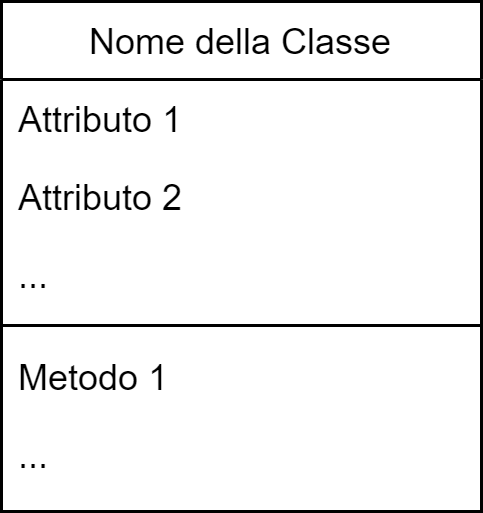
\includegraphics[width=0.25\textwidth]{classe.png}
        \caption{Rappresentazione di una classe.}
    \end{figure}
    \vspace{2mm}
     Di seguito vengono elencate tutte le possibili relazioni:
     \begin{itemize}
        \item \textbf{Dipendenza}: La relazione di dipendenza tra due classi è rappresentata da una freccia tratteggiata con la punta, che parte dalla classe dipendente A e punta alla classe da cui si origina la dipendenza B. Questa freccia indica che eventuali modifiche nella classe B potrebbero influenzare o avere un impatto sulla classe A;
        \begin{figure}[H]
            \centering
            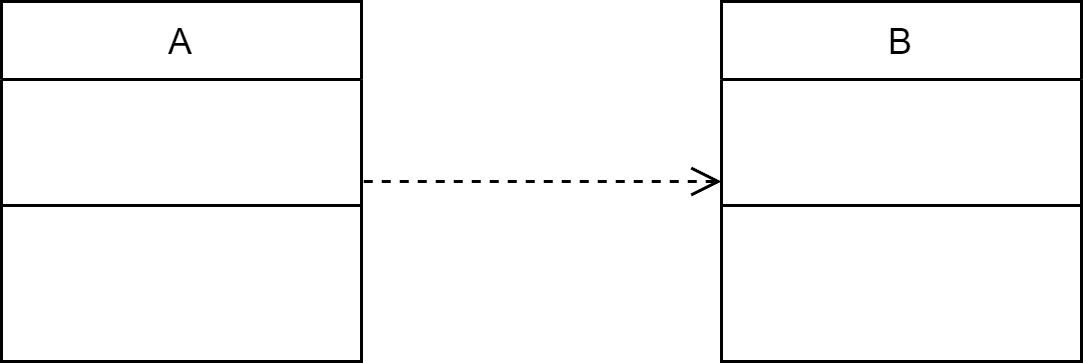
\includegraphics[width=0.5\textwidth]{dipendenza.png}
            \caption{Rappresentazione della relazione di dipendenza.}
        \end{figure}
        
        \item \textbf{Aggregazione}: La relazione di aggregazione rappresenta un legame di tipo "part of" tra due classi, in cui una classe è associata ad un'altra ma può esistere anche indipendentemente da essa. Questa relazione viene utilizzata quando una classe A (contenitore) contiene un riferimento ad un oggetto di tipo B (contenuto). L'aggregazione è rappresentata graficamente con una linea che collega le due classi, con un rombo vuoto posto vicino alla classe che rappresenta il contenitore;
        \begin{figure}[H]
            \centering
            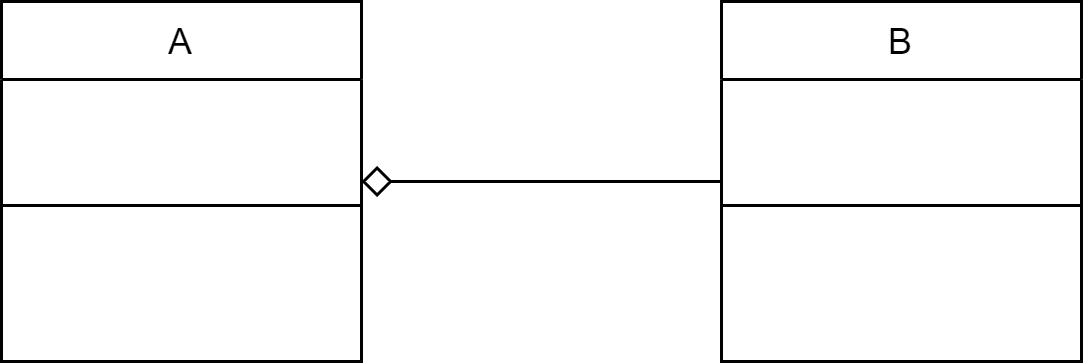
\includegraphics[width=0.5\textwidth]{aggregazione.png}
            \caption{Rappresentazione della relazione di aggregazione.}
        \end{figure}
        
        \item \textbf{Composizione}: La relazione di composizione si verifica quando una classe A contiene un oggetto di tipo B e ne ha la responsabilità di crearne e gestirne l'esistenza. La vita di B (contenuto) è vincolata a quella di A (contenitore): se A viene eliminata, anche B viene distrutta. La composizione è rappresentata graficamente con un rombo pieno vicino alla classe che rappresenta il contenitore e una linea che collega le due classi;
        \begin{figure}[H]
            \centering
            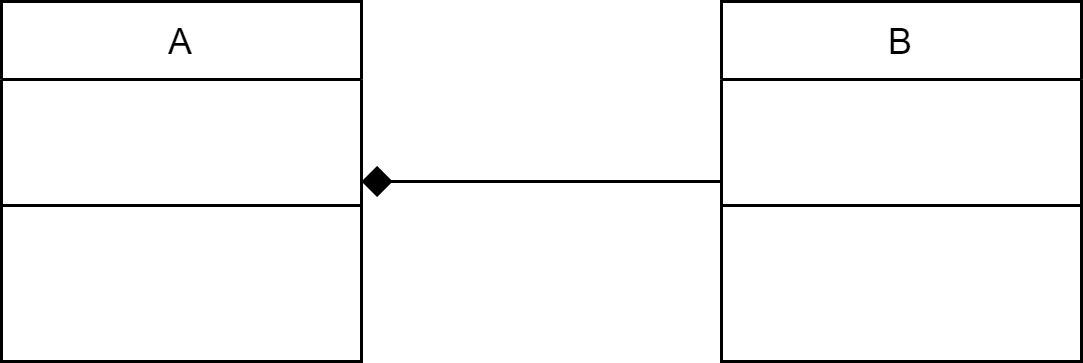
\includegraphics[width=0.5\textwidth]{composizione.png}
            \caption{Rappresentazione della relazione di composizione.}
        \end{figure}
        
        \item \textbf{Associazione}: La relazione di associazione si verifica quando una classe può contenere riferimenti o istanze di un’altra classe senza implicare una stretta dipendenza. L'associazione è rappresentata graficamente con una linea che collega le classi, spesso accompagnata da valori di molteplicità. Per indicare il senso della relazione, può essere utilizzata una freccia posizionata su uno dei due estremi;
        \begin{figure}[H]
            \centering
            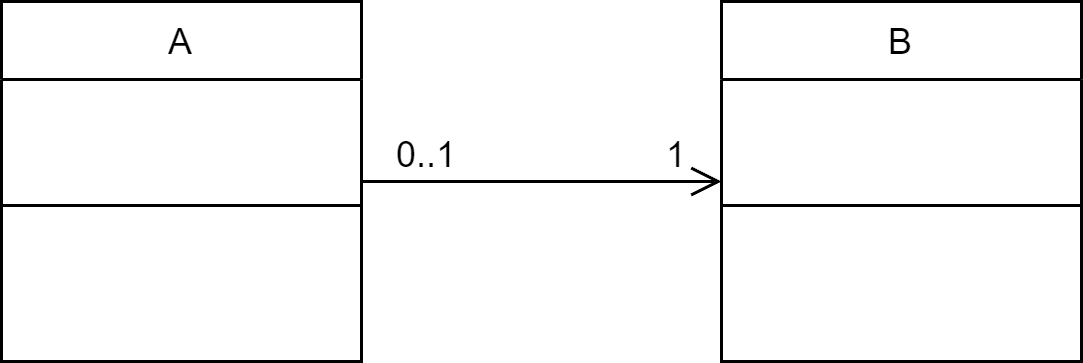
\includegraphics[width=0.5\textwidth]{associazione_classe.png}
            \caption{Rappresentazione della relazione di associazione.}
        \end{figure}
        
        \item \textbf{Generalizzazione}: La relazione di generalizzazione si verifica quando una classe eredita attributi, comportamenti e relazioni dalla classe genitore. Nello specifico ogni istanza della classe figlia è anche un'istanza della classe genitore, ma con caratteristiche o dettagli aggiuntivi specifici. La generalizzazione è rappresentata graficamente con una freccia vuota che collega la classe figlia (B) alla classe genitore (A);
        \begin{figure}[H]
            \centering
            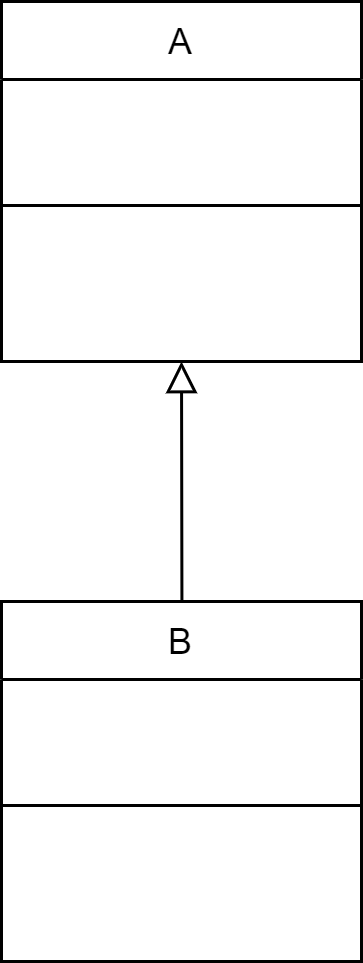
\includegraphics[width=0.2\textwidth]{generalizzazione.png}
            \caption{Rappresentazione della relazione di generalizzazione.}
        \end{figure}
     \end{itemize}
    
    \paragraph{Metriche}
    %da completare e inserire tabella%

    
    \subsubsection{Codifica}

    \paragraph{Descrizione e scopo} 
    L’attività di codifica rappresenta la fase cruciale in cui le funzionalità richieste dal proponente vengono tradotte in istruzioni eseguibili. I Programmatori, incaricati di questa attività, hanno il compito di implementare il design concettuale definito dai Progettisti, seguendo scrupolosamente le linee guida e le norme stabilite. Questo metodo di lavoro garantisce che il codice segua accuratamente le specifiche, promuovendo qualità, mantenibilità e coerenza nell’intero progetto.\\
    L’obiettivo principale della codifica è quindi creare un prodotto software che soddisfi le esigenze del proponente e rispetti gli accordi contrattuali. Le aspettative del codice sviluppato includono:
    \begin{itemize}
        \item \textbf{Conformità alle specifiche}: garantire che il codice traduca fedelmente i requisiti e le funzionalità richieste;
        \item \textbf{Chiarezza e leggibilità}: scrivere codice autoesplicativo, riducendo la necessità di commenti superflui;
        \item \textbf{Ottimizzazione delle prestazioni}: assicurare che il codice sia efficiente e scalabile;
        \item \textbf{Testabilità}: integrare test di unità e di integrazione per verificare la correttezza e l’affidabilità;
    \end{itemize}
    
    \paragraph{Norme di codifica}
    Per garantire uno sviluppo del codice coerente e di alta qualità, i Programmatori adottano le seguenti regole:
    \begin{itemize}
        \item \textbf{Nomi significativi}: utilizzare nomi univoci, oltre che chiari e descrittivi per variabili, metodi e classi, evitando abbreviazioni ambigue;
        \item \textbf{Indentazione}: applicare uno schema di formattazione uniforme per migliorare la leggibilità del codice. Ogni livello di annidamento deve essere chiaramente separato con un tab o spazi coerenti;
        \item \textbf{Lunghezza dei metodi}: i metodi devono essere brevi e focalizzati su una singola responsabilità, per favorire test di unità efficaci;
    \end{itemize}
    
    \paragraph{Strumenti utilizzati}
    Il team di sviluppo utilizza strumenti che supportano la scrittura di codice leggibile, mantenibile e conforme agli standard. Tra questi:
    \begin{itemize}
        \item \textbf{Visual Studio Code}: l'IDE principale scelto per la codifica, grazie alla sua versatilità e facilità d'uso;
    \end{itemize}
    
    \paragraph{Metriche}
    %da completare e inserire tabella%
    
    \paragraph{Integrazione}
    Durante la fase di integrazione le diverse componenti, moduli o servizi del progetto vengono combinati e testati per creare un sistema coeso e funzionante. 
    L'obiettivo principale dell'integrazione è garantire che tutte le parti del sistema interagiscano correttamente e rispettino i requisiti funzionali e di prestazione definiti. 
    Sin dalle prime fasi di sviluppo è necessario integrare le componenti del prodotto adottando un approccio solido ma flessibile, essenziale per garantire che le soluzioni esplorate durante la fase di Proof of Concept (PoC) siano utili una volta che il progetto entra nella fase di sviluppo del Minimum Viable Product (MVP). 
    Questa fase è supportata da test di integrazione che verificano che i moduli lavorino correttamente insieme. L'integrazione continua, supportata da strumenti automatizzati come CI/CD (Continuous Integration/Continuous Delivery), permette di garantire che ogni nuova modifica non comprometta l'affidabilità del sistema, mantenendo un flusso di lavoro agile e risolvendo eventuali problemi o incompatibilità prima che si presentino nel sistema finale.
    
    \paragraph{Verifica}
    La verifica è una fase cruciale del ciclo di vita del software, durante la quale si controlla che il codice sviluppato rispetti le specifiche e soddisfi i requisiti stabiliti. Questo processo garantisce che il prodotto sia conforme agli standard di qualità, riducendo al minimo la presenza di errori e assicurando un’implementazione efficiente e mantenibile. 
    Il processo di verifica comprende sia un’analisi statica del codice, per rilevare eventuali errori o problemi di formattazione, sia l’esecuzione di test mirati per validare le funzionalità implementate.


